%What is Giraf?
%What is the point of the project?

% chapter Giraf semester project (end)
The following section briefly describes what the Giraf project is and it's development. The primary source of information for this section is information from the Giraf website\cite{GirafWebsite}.


Giraf is a project that focuses on making a digital tablet environment to use as a tool for autistic people with limited verbal communication skills. The project is developed by software engineering students, as part of their bachelor projects.  The software engineering students work in small teams and coordinate the work between the teams. The project is in collaboration with the following institutes:

\begin{itemize}
    \item Børnehaven Birken (Kindergarten) \cite{bhBirken} 
    \item Egebakken (School) \cite{egebakken} 
    \item Enterne (Home for disabled) \cite{enterne}
    \item The speech institute at Aalborg municipality %verify the existence of this institute
    \item Center for Autism and ADHD \cite{center_for_autism}
\end{itemize} 
The project has run since 2011, and each year, the students continue where the last year students left off.

At the beginning of the project, it was decided to, like previous years, run the project with the \gls{Scrum_principles}. One group was appointed \gls{PO} team, and another was appointed Scrum master team. The \gls{PO} team had the responsibility of talking to the costumer, and making the product backlog. The Scrum master team had the responsibility of deciding  and facilitate how the collaboration in the project should run, and witch guidelines the groups had to follow. 

\section{Current state of Giraf}

Over the years the Giraf project has run, many different apps has been developed. However, when many different groups, works on the same project throughout multiple years,  has resulted in some problems. \newline
These problems comes from different ideas, coding styles, and an incomplete mental model of the system, and has resulted in an incoherent structure of the program.  \newline
This also had the effect, that only one app, named Weekplanner, works at this time. This is because the groups in 2017 \cite{SW608F18} changed the backend of the system, leaving all apps unusable, and then only had time to update the Weekplanner application. \newline
However, this is the only app that has been worked on the last couple of years, and after talking to the costumer, the \gls{PO} group also decided to only work on the Weekplanner app.  \newline 

\par \noindent
%Over the years the Giraf project has run, many different apps has been developed. However, at this time, only one app works. This app is called the Weekplanner. This is a result of changes to the backend without consideration of the structure of the other apps\cite{AppsStatus2019}.  \newline
The weekplanner, however, is the only app that has been focus on in the last years. After the \gls{PO} group talked to the costumer, it was decided to continue this focus on the Weekplanner this year. Thus, this is the only app that will be described in this report.  \newline
The weekplanner app is meant as a tool for showing autistic people what they will do for a week. Each day has activities associated with it, each of them represented as a picture also called a pictogram. The activities are then ordered the first being on top, and later activities going down. The state of the app from the start of 2019, can be seen in \autoref{fig:WeekPlannerPicture}.

\begin{figure}[ht]
        \begin{center}
            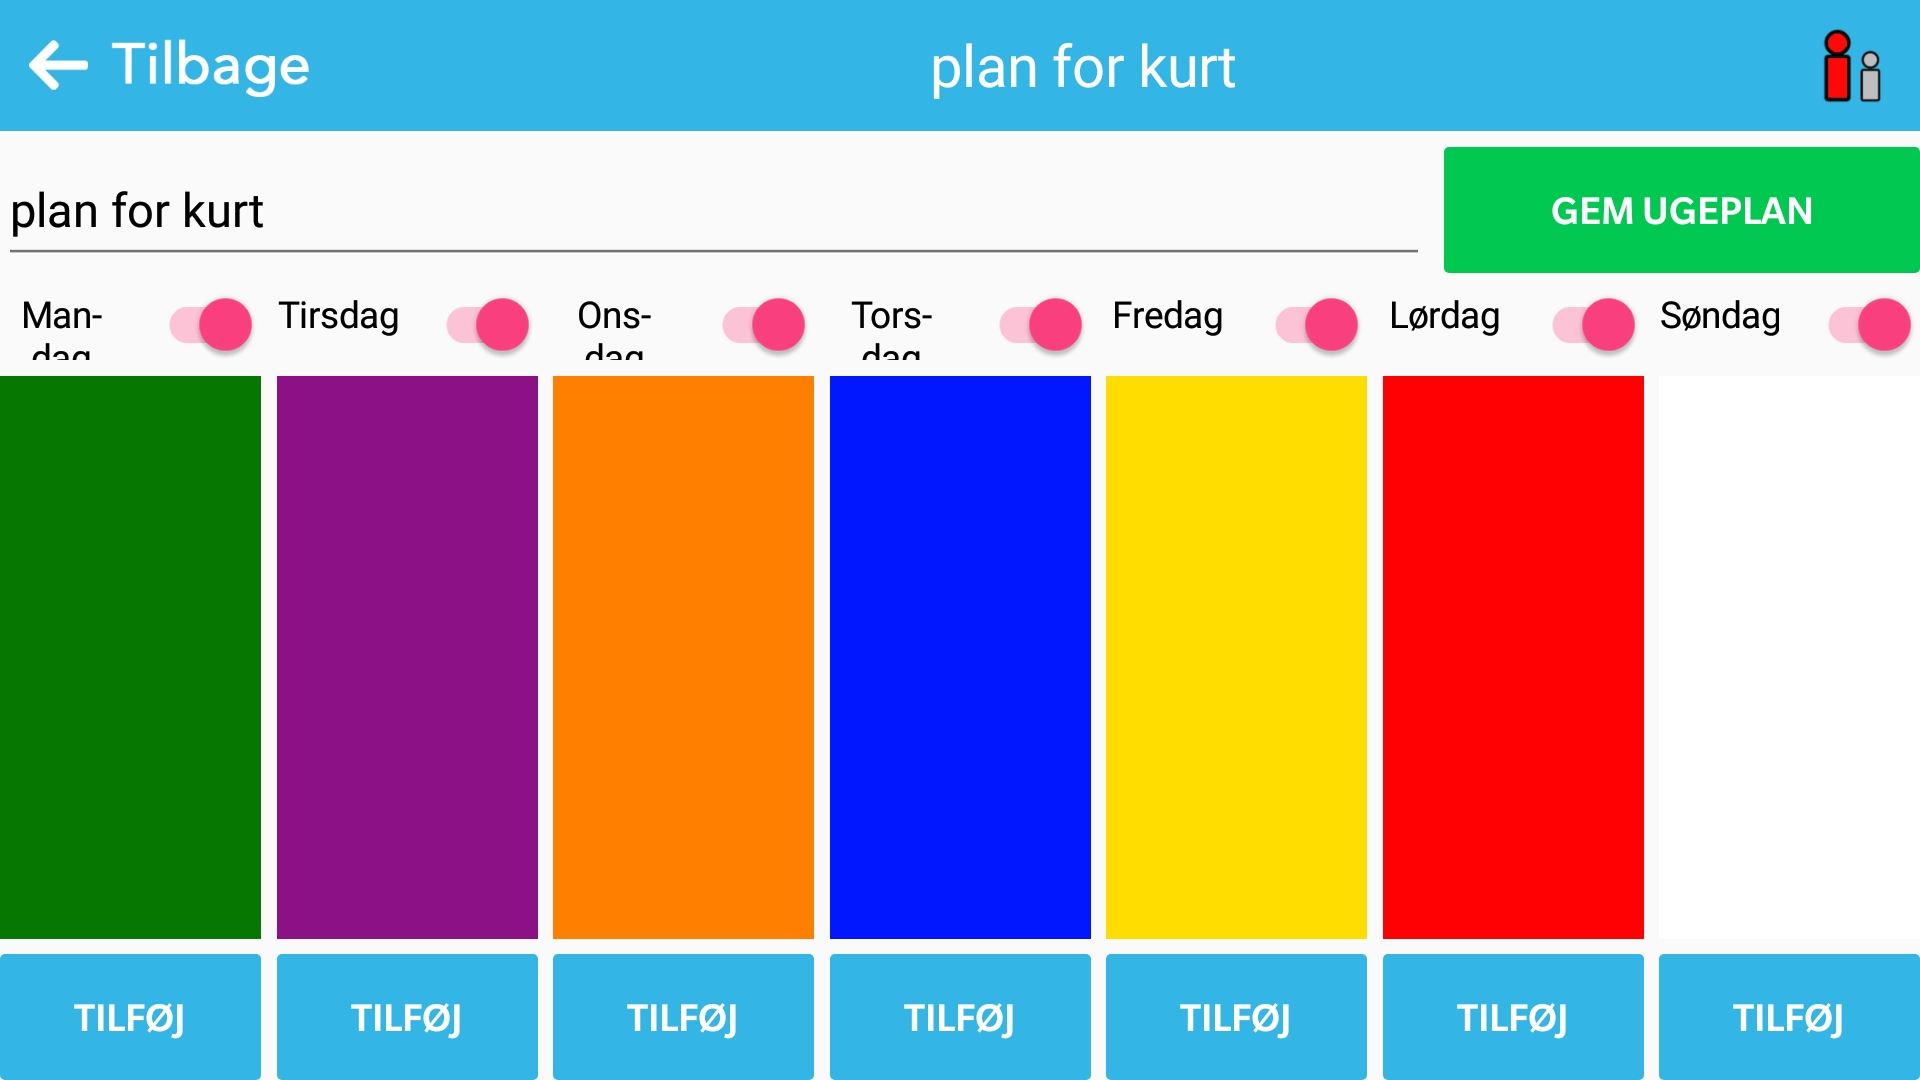
\includegraphics[width=0.95\textwidth]{figures/WeekPlannerPicture}
        \end{center}
        \caption{Weekplanner state at the start of 2019}
        \label{fig:WeekPlannerPicture}
\end{figure}

\noindent
The weekplanner app is currently running Xamarin, and can run on both android and IOS devices. The frontend of the app is build with the \gls{Mvvm} pattern. 
Backend is... %Jeg er ikke helt sikker på det her, vide mere for at skrive. 
